%
% overall.tex
%
% Copyright (C) 2021 by SpaceLab.
%
% FloripaSat-2 Documentation
%
% This work is licensed under the Creative Commons Attribution-ShareAlike 4.0
% International License. To view a copy of this license,
% visit http://creativecommons.org/licenses/by-sa/4.0/.
%

%
% \brief Overall description chapter.
%
% \author Gabriel Mariano Marcelino <gabriel.mm8@gmail.com>
%
% \institution Universidade Federal de Santa Catarina (UFSC)
%
% \version 0.1.0
%
% \date 2020/06/05
%

\chapter{Overall Description} \label{ch:overall}

.

\section{General Diagrams}

The CubeSat's subsystems are positioned in the 2U physical structure as exemplified in \autoref{fig:subsystems-positioning}. An exploded 3D view of the satellite is showed in \autoref{fig:exploded-view}.

\begin{figure}[!ht]
    \begin{center}
        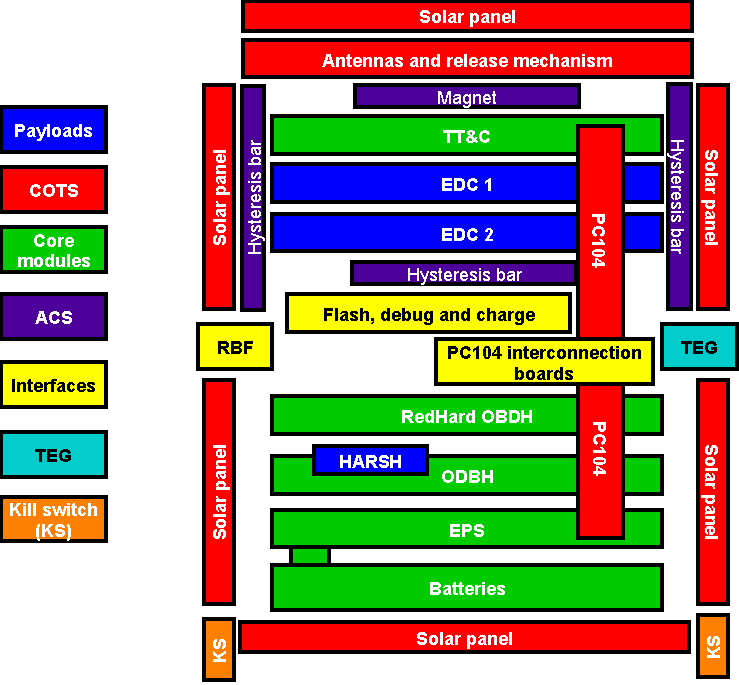
\includegraphics[width=0.7\textwidth]{figures/subsystems-positioning.pdf}
        \caption{Subsystems positioning.}
        \label{fig:subsystems-positioning}
    \end{center}
\end{figure}

%   TBD 
%   In \autoref{fig:datapath-diagram} there is a block diagram showing the satellite modules and the internal communication interfaces.

\section{General Behaviour}

.

\section{Orbit Parameters}

GMAT\nomenclature{\textbf{GMAT}}{\textit{General Mission Analysis Tool.}} \cite{gmat}

\cite{marino2016}

\begin{table}[!h]
    \centering
    \begin{tabular}{lcc}
        \toprule[1.5pt]
        \textbf{Parameters} & \textbf{Value} & \textbf{Unit} \\
        \midrule
        Altitude                & 550           & km \\
        Eccentricity            & 0,0015051     & $^{\circ}$ \\
        Inclination             & 97,9750       & $^{\circ}$ \\
        RAAN                    & 85,5100       & $^{\circ}$ \\
        Arg. of Perigee (AOP)   & 194,87        & $^{\circ}$ \\
        TA                      & 99,8877       & $^{\circ}$ \\
        \bottomrule[1.5pt]
    \end{tabular}
    \caption{Initial orbit parameters (adapter from FloripaSat-I).}
    \label{tab:orbit-parameters}
\end{table}

The following parameters were chosen for the setup of GMAT software:

\begin{itemize}
    \item Force model for gravitational field: ``\textit{Earth Gravitational Model 1996 (EGM96)}''
    \item Propagator: ``\textit{PrinceDorman78}''
    \item Drag coefficient: 2,2
    \item Drag atmosphere model: ``\textit{Mass Spectrometry and Incoherent Scatter (MSISE90)}''
\end{itemize}

\begin{figure}[!ht]
    \begin{center}
        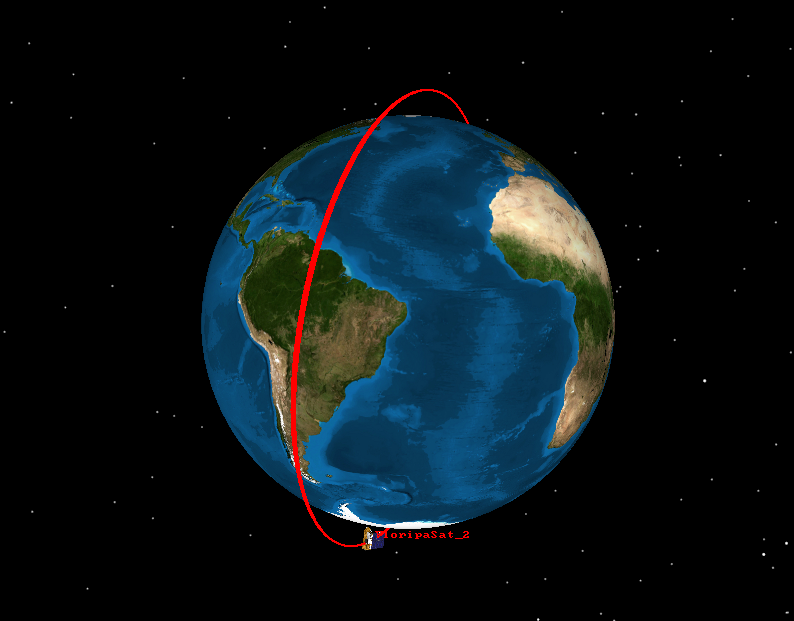
\includegraphics[width=0.6\textwidth]{figures/fsat2-gmat.png}
        \caption{FloripaSat-2 orbit simulation on GMAT.}
        \label{fig:fsat2-gmat}
    \end{center}
\end{figure}

\begin{figure}[!ht]
    \begin{center}
        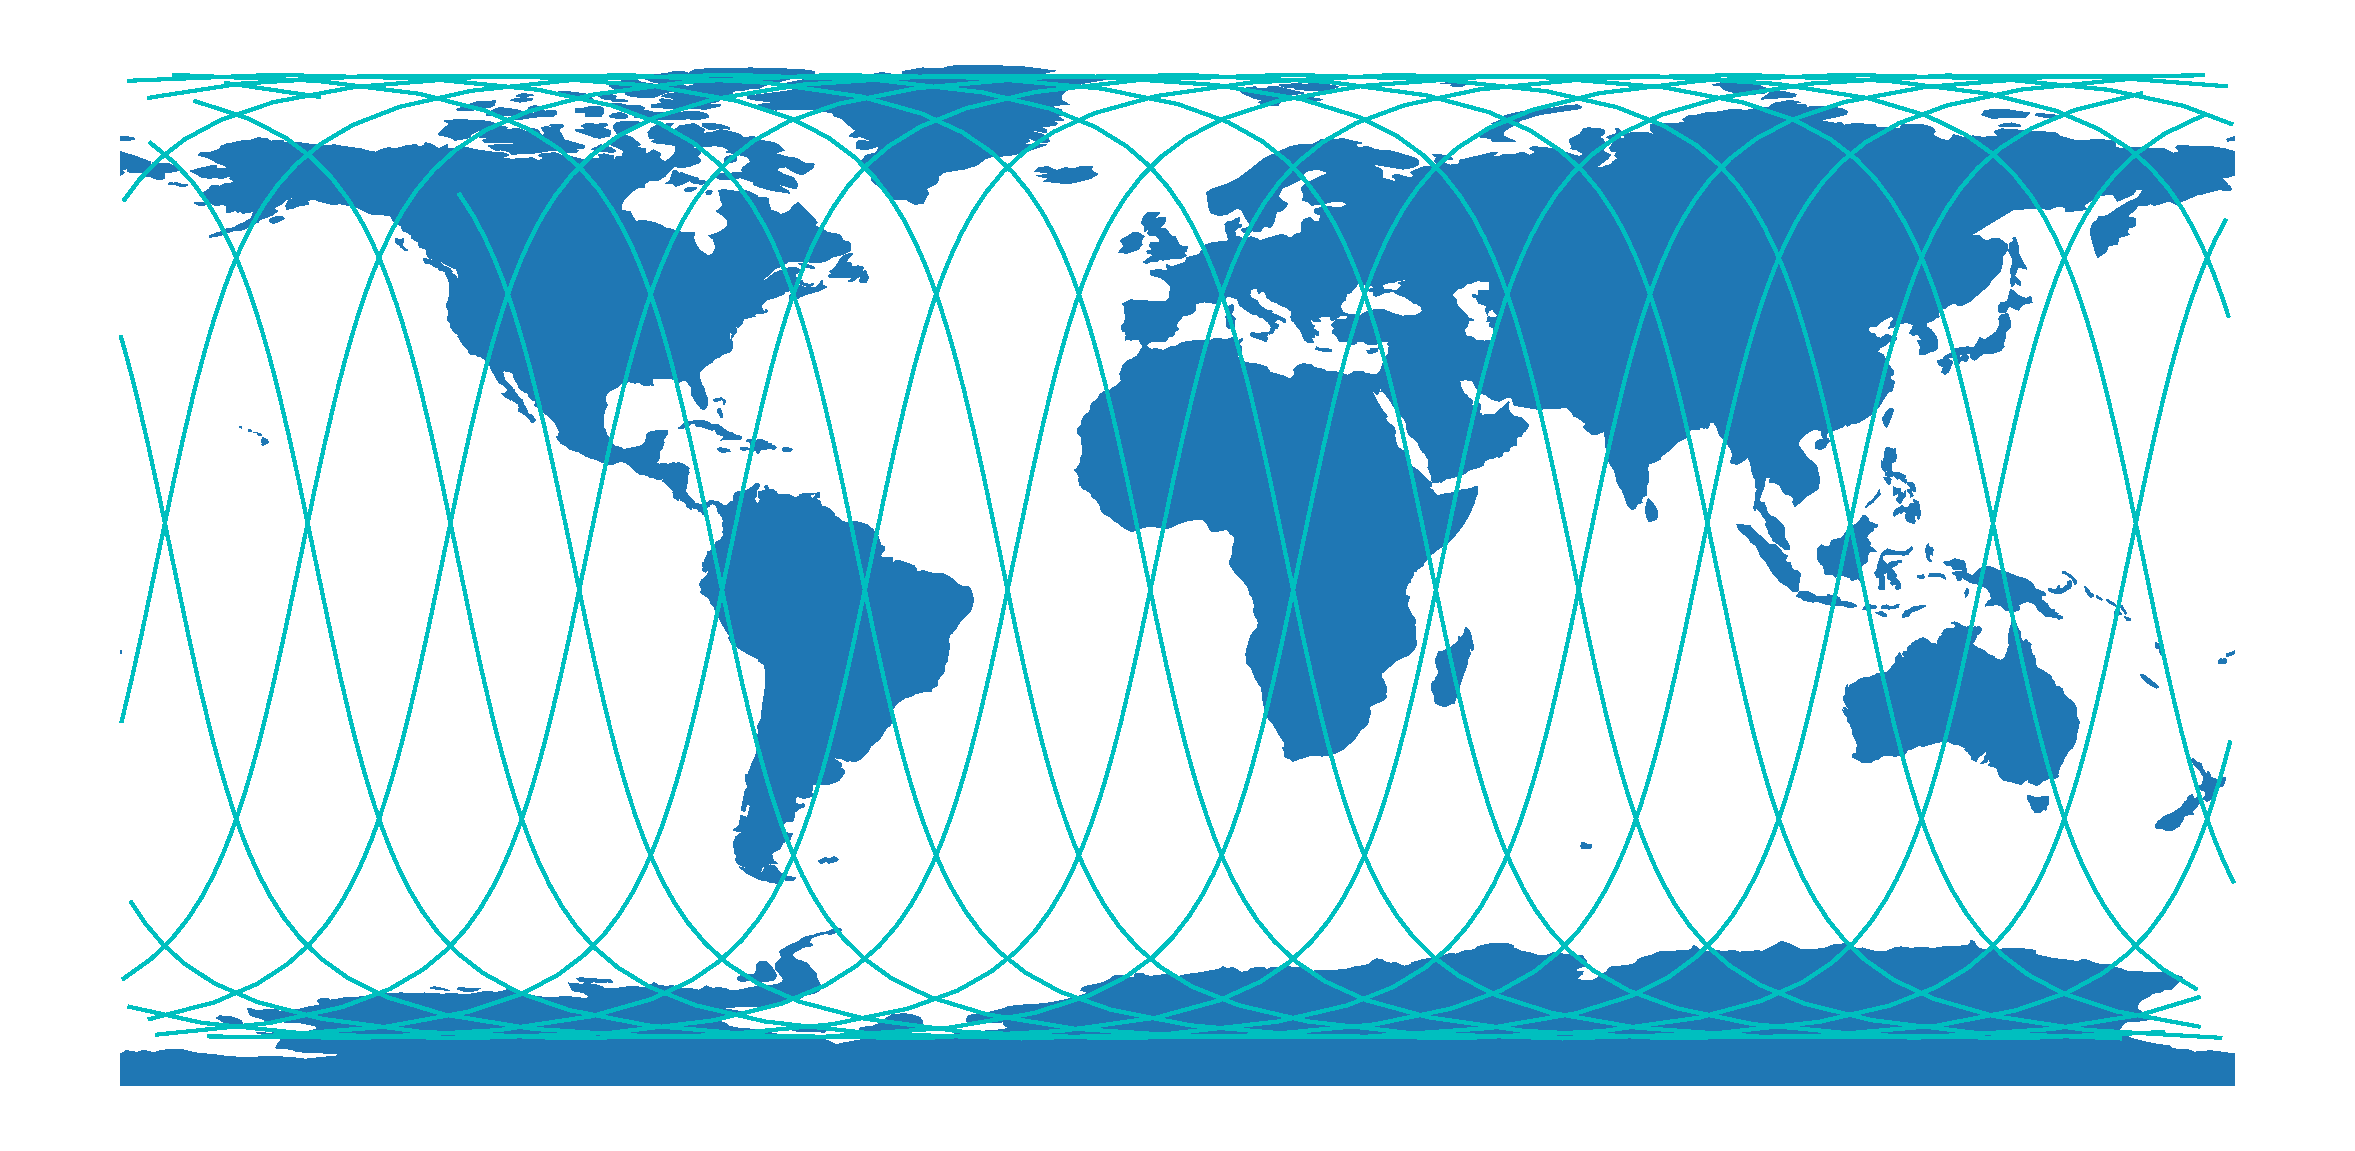
\includegraphics[width=\textwidth]{figures/fsat2-gmat-groundtrack.pdf}
        \caption{FloripaSat-2 simulated groundtrack.}
        \label{fig:fsat2-gmat-groundtrack}
    \end{center}
\end{figure}

\subsection{Lifetime Analysis}

Considering the same parameters of FloripaSat-I, but with an initial altitude of 550 km, the simulations on GMAT showed that the satellite decays approximately in 2000 days ($\cong$ 5 years), as can be seen in \autoref{fig:lifetime-analysis}.

\begin{figure}[!ht]
    \begin{center}
        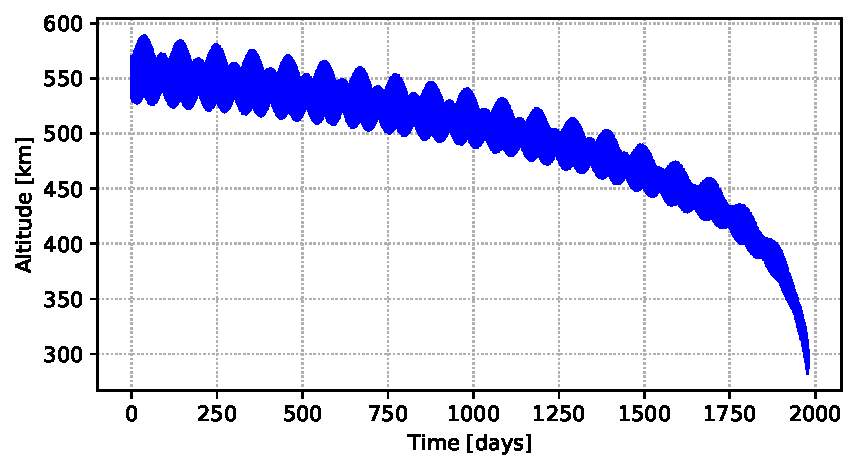
\includegraphics[width=\textwidth]{curves/lifetime.pdf}
        \caption{Lifetime analysis on GMAT.}
        \label{fig:lifetime-analysis}
    \end{center}
\end{figure}

\subsection{Ground Station Passes and Data Transfer Analysis}

Considering two ground stations, one at the SpaceLab installations in Florianópolis (27$^{\circ}$ 36' 00.9" S, 48$^{\circ}$ 31' 03.2" W) and other at the INPE/CRN installations in Natal (5$^{\circ}$ 50' 10.1" S, 35$^{\circ}$ 12' 27.5" W), both with a minimum elevation of 15$^{\circ}$, the following results were achieved during the simulations on GMAT (\autoref{tab:grs-contacts-analysis}).

\begin{table}[!h]
    \centering
    \begin{tabular}{lccc}
        \toprule[1.5pt]
        \textbf{Parameter} & \textbf{UFSC Station} & \textbf{INPE-RN Station} & \textbf{Unit} \\
        \midrule
        Minimum elevation to a valid contact    & 15    & 15    & $^{\circ}$ \\
        Number of contacts                      & 143   & 125   & - \\
        Minimum contact period                  & 24    & 34    & sec \\
        Maximum contact period                  & 395   & 394   & sec \\
        Average contact period                  & 303   & 298   & sec \\
        Total contact period                    & 43394 & 37205 & sec \\
        \bottomrule[1.5pt]
    \end{tabular}
    \caption{Ground station contacts analysis during the first 60 days of operation.}
    \label{tab:grs-contacts-analysis}
\end{table}

As can be seen from \autoref{tab:grs-contacts-analysis}, during the first 60 days of operation, considering the two main ground stations that will contact the satellite, the total contact period is 80599 seconds (43394 + 37205). With the data rate of the downlink/uplink as 4800 bps, this time period will allow a data transfer of 48359400 bytes (or 46,12 M$_{i}$B) between FloripaSat-2 and the Earth. Using the lifetime of the satellite from the previous analysis (2000 days), and an average data transfer per day of 805990 bits, the total theoretical raw data transfer during the whole operation of the satellite will be approximately 1,5 G$_{i}$B.

These values can be even bigger if a smaller minimum elevation is considered.

\section{Power Budget}

.

\section{Link Budget}

The link budget of all radio links of the satellite is available in \autoref{tab:link-budget-results}.

\begin{table}[!h]
    \centering
    \begin{tabular}{L{0.3\textwidth}ccccc}
        \toprule[1.5pt]
        \textbf{Variable} & \textbf{Beacon} & \textbf{Downlink} & \textbf{Uplink} & \textbf{Uplink (Payload)} & \textbf{Unit}\\
        \midrule
        Frequency                       & 145,97    & 436,9     & 436,9     & 401,635   & MHz \\
        Modulation                      & GMSK      & GMSK      & GMSK      & BPSK      & - \\
        Protocol                        & NGHam     & NGHam     & NGHam     & SBCD      & - \\
        Transmit power                  & 30        & 30        & 47        & ??        & dBm \\
        FSPL                            & 144,8     & 154,3     & 154,3     & ??        & dB \\
        Other losses                    & 5         & 5         & 7         & 5         & dB \\
        Receive antenna gain            & 12        & 15.5      & 0         & 0         & dBi \\
        Receiver noise temp.            &           &           &           &           & K \\
        Antenna noise temp.             &           &           &           &           & K \\
        System noise temp.              &           &           &           &           & K \\
        Data rate                       & 1200      & 4800      & 4800      & 400       & bps \\
        Received SNR                    & 30,87     & 17,35     & 31,60     & ??        & dB \\
        SNR required for $10^{-5}$ BER*  & 9,6       & 9,6       & 9,6       & 9,6       & dB \\
        Link margin                     & $\leq$ 21,27 & $\leq$ 7,75 & $\leq$ 22 & $\leq$ ?? & dB \\
        \bottomrule[1.5pt]
    \end{tabular}
    \caption{Link budget results.}
    \label{tab:link-budget-results}
\end{table}

All equations and steps used to obtain the results of \autoref{tab:link-budget-results} are available in \autoref{anx:link-budget}.

\section{PC-104 Bus}

\begin{figure}[!ht]
    \begin{center}
        \includegraphics[width=0.5\textwidth]{figures/pc104-diagram}
        \label{fig:pc104-diagram}
        \caption{Reference diagram of the PC-104 bus.}
    \end{center}
\end{figure}

\begin{table}[!h]
    \centering
    \begin{tabular}{cllll}
        \toprule[1.5pt]
        \textbf{Pin Row}   & \textbf{H1 Odd}  & \textbf{H1 Even} & \textbf{H2 Odd} & \textbf{H2 Even} \\
        \midrule
        1-2                & -                & -                & -               & -                \\
        3-4                & -                & -                & EDC\_1\_EN      & EDC\_2\_EN       \\
        5-6                & -                & -                & BE\_UART\_RX    & -                \\
        7-8                & RA\_GPIO\_0      & RA\_GPIO\_1      & BE\_UART\_TX    & GPIO\_0          \\
        9-10               & RA\_GPIO\_2      & BE\_EN           & -               & -                \\
        11-12              & RA\_RESET        & RA\_EN           & BE\_SPI\_MOSI   & BE\_SPI\_CLK     \\
        13-14              & -                & -                & BE\_SPI\_CS     & BE\_SPI\_MISO    \\
        15-16              & -                & -                & -               & -                \\
        17-18              & EDC\_UART\_RX/TX & PLX\_EN          & -               & GPIO\_1          \\
        19-20              & EDC\_UART\_TX/RX & GPIO\_2          & -               & GPIO\_3          \\
        21-22              & -                & -                & -               & GPIO\_4          \\
        23-24              & -                & -                & -               & -                \\
        25-26              & -                & -                & PL\_VCC         & PL\_VCC          \\
        27-28              & -                & -                & TTC\_VCC        & TTC\_VCC         \\
        29-30              & GND              & GND              & GND             & GND              \\
        31-32              & GND              & GND              & GND             & GND              \\
        33-34              & -                & -                & -               & -                \\
        35-36              & RA\_SPI\_CLK     & -                & ANT\_VCC        & ANT\_VCC         \\
        37-38              & RA\_SPI\_MISO    & -                & -               & -                \\
        39-40              & RA\_SPI\_MOSI    & RA\_SPI\_CS      & -               & -                \\
        41-42              & PL\_I2C\_SDA     & -                & -               & GPIO\_5          \\
        43-44              & PL\_I2C\_SCL     & -                & -               & -                \\
        45-46              & OBDH\_VCC        & OBDH\_VCC        & BAT\_VCC        & BAT\_VCC         \\
        47-48              & PL\_VCC          & PL\_VCC          & -               & -                \\
        49-50              & RA\_VCC          & RA\_VCC          & EPS\_I2C\_SDA   & -                \\
        51-52              & BE\_VCC          & BE\_VCC          & EPS\_I2C\_SCL   & -                \\
        \bottomrule[1.5pt]
    \end{tabular}
    \caption{PC-104 bus pinout.}
    \label{tab:pc104-pinout}
\end{table}

\begin{table}[!h]
    \centering
    \begin{tabular}{lL{0.18\textwidth}L{0.17\textwidth}L{0.33\textwidth}}
        \toprule[1.5pt]
        \textbf{Signal}  & \textbf{Pin(s)} & \textbf{Used By}     & \textbf{Description} \\
        \midrule
        GND              & H1-29/30/31/32, H2-29/30/31/32 & All   & Ground reference \\
        BAT\_VCC         & H2-45, H2-46    & EPS                  & Battery terminals (+) \\
        ANT\_VCC         & H2-35, H2-36    & EPS, ANT             & Antenna power supply (3.3 V) \\
        OBDH\_VCC        & H1-45, H1-46    & EPS, OBDH            & OBDH power supply (3.3 V) \\
        TTC\_VCC         & H2-27, H2-28    & EPS, TTC             & TTC power supply (3.3 V) \\
        PL\_VCC          & H1-47/48, H2-25/26 & EPS, EDC 1/2, Payload X & Payloads power supply (5 V) \\
        RA\_VCC          & H1-49, H1-50    & EPS, TTC             & Main radio power supply (5 V) \\
        BE\_VCC          & H1-51, H1-52    & EPS, TTC             & Beacon power supply (6 V) \\
        RA\_SPI\_CLK     & H1-35           & OBDH, TTC            & CLK signal of the main radio SPI bus \\
        RA\_SPI\_MISO    & H1-37           & OBDH, TTC            & MISO signal of the main radio SPI bus \\
        RA\_SPI\_MOSI    & H1-39           & OBDH, TTC            & MOS signal of the main radio SPI bus \\
        RA\_SPI\_CS      & H1-40           & OBDH, TTC            & CS signal of the main radio SPI bus \\
        EPS\_I2C\_SDA    & H2-49           & OBDH, EPS            & SDA signal of the EPS I2C bus \\
        EPS\_I2C\_SCL    & H2-51           & OBDH, EPS            & SCL signal of the EPS I2C bus \\
        BE\_UART\_RX     & H2-5            & EPS, TTC             & EPS TX, Beacon RX (UART bus) \\
        BE\_UART\_TX     & H2-7            & EPS, TTC             & EPS RX, Beacon TX (UART bus) \\
        EDC\_UART\_TX/RX & H1-25           & OBDH, EDC 1/2        & OBDH TX, EDCs RX (UART bus) \\
        EDC\_UART\_RX/TX & H1-27           & OBDH, EDC 1/2        & OBDH RX, EDCs TX (UART bus) \\
        BE\_EN           & H1-10           & EPS, TTC             & Beacon radio power enable \\
        RA\_EN           & H1-12           & EPS, OBDH            & Main radio power enable \\
        EDC\_1\_EN       & H2-3            & OBDH, EDC 1          & EDC 1 enable signal \\
        EDC\_2\_EN       & H2-4            & OBDH, EDC 2          & EDC 2 enable signal \\
        PLX\_EN          & H1-18           & OBDH, Payload X      & Payload X enable (GPIO) \\
        PL\_I2C\_SDA     & H1-41           & OBDH, Payload X      & SDA signal of the payload I2C bus \\
        PL\_I2C\_SCL     & H1-43           & OBDH, Payload X      & SCL signal of the payload I2C bus \\
        GPIO\_N          & H1-20, H2-8/18/20/22/42  & OBDH        & GPIO pin (not used) \\
        \bottomrule[1.5pt]
    \end{tabular}
    \caption{PC-104 bus signal description.}
    \label{tab:pc104-signals}
\end{table}

\section{Telecommunication}

\begin{landscape}
    \begin{table}[ht]
        \centering
        \begin{tabular}{llccccc}
            \toprule[1.5pt]
            \multirow{2}{*}{\textbf{Link}} & \multirow{2}{*}{\textbf{Packet Name}} & \multicolumn{4}{c}{\textbf{Payload}} & \multirow{2}{*}{\textbf{Access}} \\
            \cmidrule{3-6}
                                      &                       & \textbf{ID}  & \textbf{Source Callsign}   & \textbf{Data (up to 220 bytes)}            & \textbf{Size (bytes)} & \\
            \midrule
            \multirow{2}{*}{Beacon}   & EPS data              & 00h & \multirow{2}{*}{``0'' + ``PY0EGU''} & EPS data                                   & 58                    & Public \\
                                      & TTC Data              & 01h &                                     & TTC data                                   & 18                    & Public \\
            \midrule
            \multirow{8}{*}{Downlink} & Telemetry             & 20h & \multirow{8}{*}{``0'' + ``PY0EGU''} & Flags + OBDH/EPS data                      & 220                   & Public \\
                                      & Ping answer           & 21h &                                     & Requester callsign                         & 15                    & Public \\
                                      & Data request answer   & 22h &                                     & Req. callsign + data                       & 15 to 155             & Public \\
                                      & Message broadcast     & 23h &                                     & Req. + dst. callsign + message             & 22 to 60              & Public \\
                                      & Hibernation feedback  & 24h &                                     & Req. callsign + hibernation in hours       & 17                    & Public \\
                                      & EDC info              & 25h &                                     & PTT decoder + HK info + system state       & 79                    & Public \\
                                      & EDC samples           & 26h &                                     & Timestamp + pkt. counter + samples         & 219                   & Public \\
                                      & TC feedback           & 27h &                                     & Req. callsign + TC packet ID + timestamp   & 13                    & Public \\
            \midrule
            \multirow{14}{*}{Uplink}  & Ping Request          & 40h & \multirow{14}{*}{Any Callsign}      & None                                       & 8                     & Public \\
                                      & Data Request          & 41h &                                     & Data flags + count + origin + offset       & 16                    & Public \\
                                      & Broadcast Message     & 42h &                                     & Dst. callsign + message                    & 15 to 46              & Public \\
                                      & Enter hibernation     & 43h &                                     & Req. callsign + hibernation in hours + key & 29                    & Private \\
                                      & Leave hibernation     & 44h &                                     & Command key                                & 16                    & Private \\
                                      & Activate beacon       & 45h &                                     & Command key                                & 16                    & Private \\
                                      & Deactivate beacon     & 46h &                                     & Command key                                & 16                    & Private \\
                                      & Activate downlink     & 47h &                                     & Command key                                & 16                    & Private \\
                                      & Deactivate downlink   & 48h &                                     & Command key                                & 16                    & Private \\
                                      & Activate EDC          & 49h &                                     & Command key                                & 16                    & Private \\
                                      & Deactivate EDC        & 4Ah &                                     & Command key                                & 16                    & Private \\
                                      & Activate Payload X    & 4Bh &                                     & Command key                                & 16                    & Private \\
                                      & Deactivate Payload X  & 4Ch &                                     & Command key                                & 16                    & Private \\
                                      & Get EDC info          & 4Dh &                                     & Command key                                & 16                    & Private \\
            \bottomrule[1.5pt]
        \end{tabular}
        \caption{Telecommunication packets and their content.}
        \label{tab:packets-struct}
    \end{table}
\end{landscape}

\begin{table}[ht]
    \centering
    \begin{tabular}{lcL{0.53\textwidth}c}
        \toprule[1.5pt]
        \textbf{Packet} & \textbf{Position} & \textbf{Content} & \textbf{Length [bytes]} \\
        \midrule
        \multirow{22}{*}{EPS data} & 0  & Packet ID (00h)                       & 1 \\
                                   & 1  & Source callsign (``0PY0EGU'')         & 7 \\
                                   & 8  & Timestamp in ms                       & 4 \\
                                   & 12 & Battery cell 1 voltage in mV          & 2 \\
                                   & 14 & Battery cell 2 voltage in mV          & 2 \\
                                   & 16 & Battery current in mA                 & 2 \\
                                   & 18 & Battery charge in mAh                 & 2 \\
                                   & 20 & Battery cell 1 temperature in K       & 2 \\
                                   & 22 & Battery cell 2 temperature in K       & 2 \\
                                   & 24 & Battery monitor temperature in K      & 2 \\
                                   & 26 & Solar panel voltage in mV (-Y and +X) & 2 \\
                                   & 28 & Solar panel voltage in mV (-X and +Z) & 2 \\
                                   & 30 & Solar panel voltage in mV (-Z and +Y) & 2 \\
                                   & 32 & Solar panel current in mA (-Y)        & 2 \\
                                   & 34 & Solar panel current in mA (+Y)        & 2 \\
                                   & 36 & Solar panel current in mA (-X)        & 2 \\
                                   & 38 & Solar panel current in mA (+X)        & 2 \\
                                   & 40 & Solar panel current in mA (-Z)        & 2 \\
                                   & 42 & Solar panel current in mA (+Z)        & 2 \\
                                   & 44 & Temperature of the EPS $\mu$C in K    & 2 \\
        \cmidrule{4-4}
                                   &    &                                       & 46 \\
        \midrule
        \multirow{9}{*}{TTC data}  & 0  & Packet ID (01h)                       & 1 \\
                                   & 1  & Source callsign (``0PY0EGU'')         & 7 \\
                                   & 8  & Timestamp in ms                       & 4 \\
                                   & 12 & Temperature of the TTC $\mu$C in K    & 2 \\
                                   & 14 & Reset counter                         & 2 \\
                                   & 16 & Last reset cause                      & 1 \\
                                   & 15 & Temperature of the beacon radio in K  & 2 \\
        \cmidrule{4-4}
                                   &    &                                       & 19 \\
        \bottomrule[1.5pt]
    \end{tabular}
    \caption{Beacon packets.}
    \label{tab:beacon-packets}
\end{table}
